% Provides macros manipulating strings of tokens.
\RequirePackage{xstring}

% Store the jobname as a string with category 11 characters.
\edef\normaljobname{\expandafter\scantokens\expandafter{\jobname\noexpand}}
\StrBehind{\normaljobname}{exer-}[\exercisenumber]

\documentclass[
  coursecode={CMPE 251},
  assignmentname={Exercise \exercisenumber},
  studentnumber=20053722,
  name={Bryan Hoang},
  final,
]{
  ltxanswer%
}

\marksnotpoints{}

\usepackage{bch-style}

\begin{document}
  \begin{questions}
    \question[2]{}
    Build a (supervised) neural network to classify the wines (Supervised neural network = multilayer perceptron = MLP in the jargon.)

    Because of the time required, use only 5-fold cross validation. Report briefly on the performance of this technique, including computational time required.

    Neural networks often perform better when their inputs are normalized, often to the interval [0,1] or [-1,+1]. Try using the Normalizer node to see if this helps.
    \begin{solution}
      \section*{Unnormalized data}
      A Supervised Neural Network (SNN) with 4 nodes in the hidden layer (\(\sqrt{13\ \text{attributes}} \approx 4\)) was built, as seen in Figure~\ref{fig:wine-workflow-unnormalized}.

      \begin{answerfigure}
        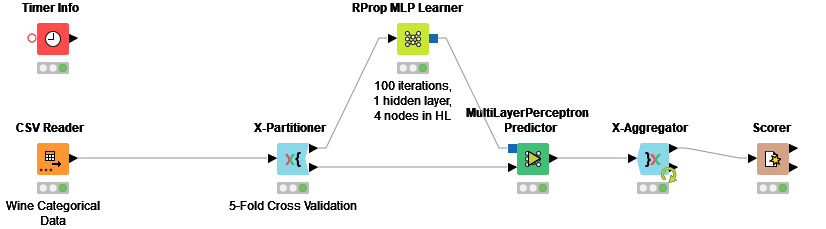
\includegraphics[width=\textwidth]{wine-workflow-unnormalized.png}
        \captionof{figure}{KNIME workflow of a SNN for unnormalized data}\label{fig:wine-workflow-unnormalized}
      \end{answerfigure}

      Based on the confusion matrix for the SNN shown in Figure~\ref{fig:wine-snn-unnormalized-confusion-matrix}, the accuracy of \qty{\sim{47}}{\percent} leaves a lot of room for improvement.

      \newpage

      \begin{answerfigure}
        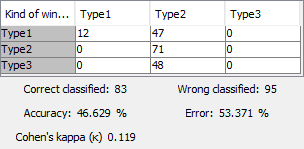
\includegraphics[width=0.66\textwidth]{wine-snn-unnormalized-confusion-matrix.png}
        \captionof{figure}{Confusion matrix of the SNN with unnormalized data}\label{fig:wine-snn-unnormalized-confusion-matrix}
      \end{answerfigure}

      Timing wise, the SNN with unnormalized data took \qty{\sim{30}}{\ms} to compute, as seen in Figure~\ref{fig:wine-snn-unnormalized-timing}.

      \begin{answerfigure}
        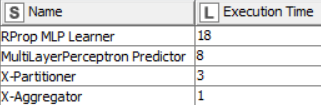
\includegraphics[width=0.66\textwidth]{wine-snn-unnormalized-timing.png}
        \captionof{figure}{Timer information for SNN with unnormalized data}\label{fig:wine-snn-unnormalized-timing}
      \end{answerfigure}

      \newpage

      \section*{Normalized data}
      \subsection*{Normalized to \([0,1]\)}
      I used the Normalizer node to normalize the data to the interval [0,1].

      \begin{answerfigure}
        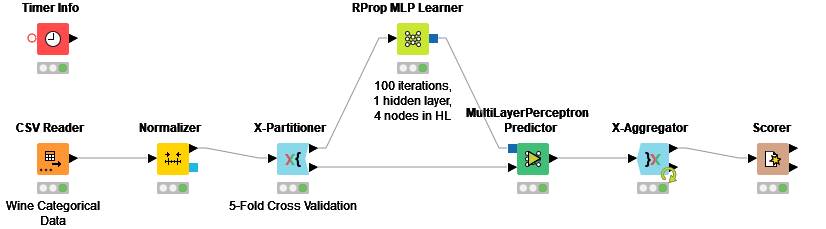
\includegraphics[width=\textwidth]{wine-workflow-normalized.png}
        \captionof{figure}{KNIME workflow of a SNN for normalized data}\label{fig:wine-workflow-normalized}
      \end{answerfigure}

      From the confusion matrix for the SNN shown in Figure~\ref{fig:wine-snn-normalized-0-1-confusion-matrix}, the accuracy of \qty{\sim{96}}{\percent} is a great \qty{39}{\percent} increase compared to using unnormalized data.

      \begin{answerfigure}
        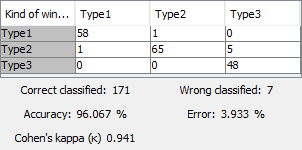
\includegraphics[width=0.66\textwidth]{wine-snn-normalized-0-1-confusion-matrix.png}
        \captionof{figure}{Confusion matrix of the SNN with data normalized to \([0,1]\)}\label{fig:wine-snn-normalized-0-1-confusion-matrix}
      \end{answerfigure}

      From Figure~\ref{fig:wine-snn-normalized-0-1-timing}, it can be seen that the SNN took \qty{\sim{42}}{\ms} to compute, which seems like an acceptable increase in execution time for the significant increase in prediction accuracy.

      \newpage

      \begin{answerfigure}
        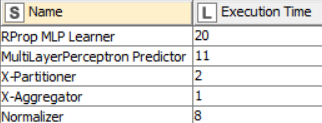
\includegraphics[width=0.66\textwidth]{wine-snn-normalized-0-1-timing.png}
        \captionof{figure}{Timer information for SNN with data normalized to \([0,1]\)}\label{fig:wine-snn-normalized-0-1-timing}
      \end{answerfigure}

      \newpage

      \subsection*{Normalized to \([-1,1]\)}

      From the confusion matrix for the SNN shown in Figure~\ref{fig:wine-snn-normalized--1-1-confusion-matrix}, the accuracy of \qty{\sim{98}}{\percent} is even better than the \qty{\sim{96}}{\percent} accuracy obtained from normalizing to the interval \([0,1]\).

      \begin{answerfigure}
        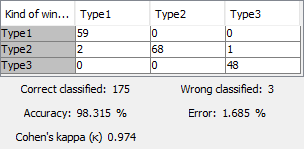
\includegraphics[width=0.66\textwidth]{wine-snn-normalized--1-1-confusion-matrix.png}
        \captionof{figure}{Confusion matrix of the SNN with data normalized to \([-1,1]\)}\label{fig:wine-snn-normalized--1-1-confusion-matrix}
      \end{answerfigure}

      From Figure~\ref{fig:wine-snn-normalized--1-1-timing}, it can be seen that the SNN took \qty{\sim{44}}{\ms} to compute, which also seems like an acceptable increase in execution time for the significant increase in prediction accuracy.

      \begin{answerfigure}
        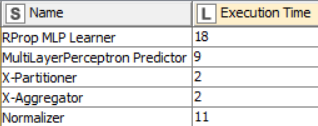
\includegraphics[width=0.66\textwidth]{wine-snn-normalized--1-1-timing.png}
        \captionof{figure}{Timer information for SNN with data normalized to \([-1,1]\)}\label{fig:wine-snn-normalized--1-1-timing}
      \end{answerfigure}
    \end{solution}
  \end{questions}
\end{document}
